\subsection{System level}
	The following graph is our system level state chart, which contains all our class level state charts.

	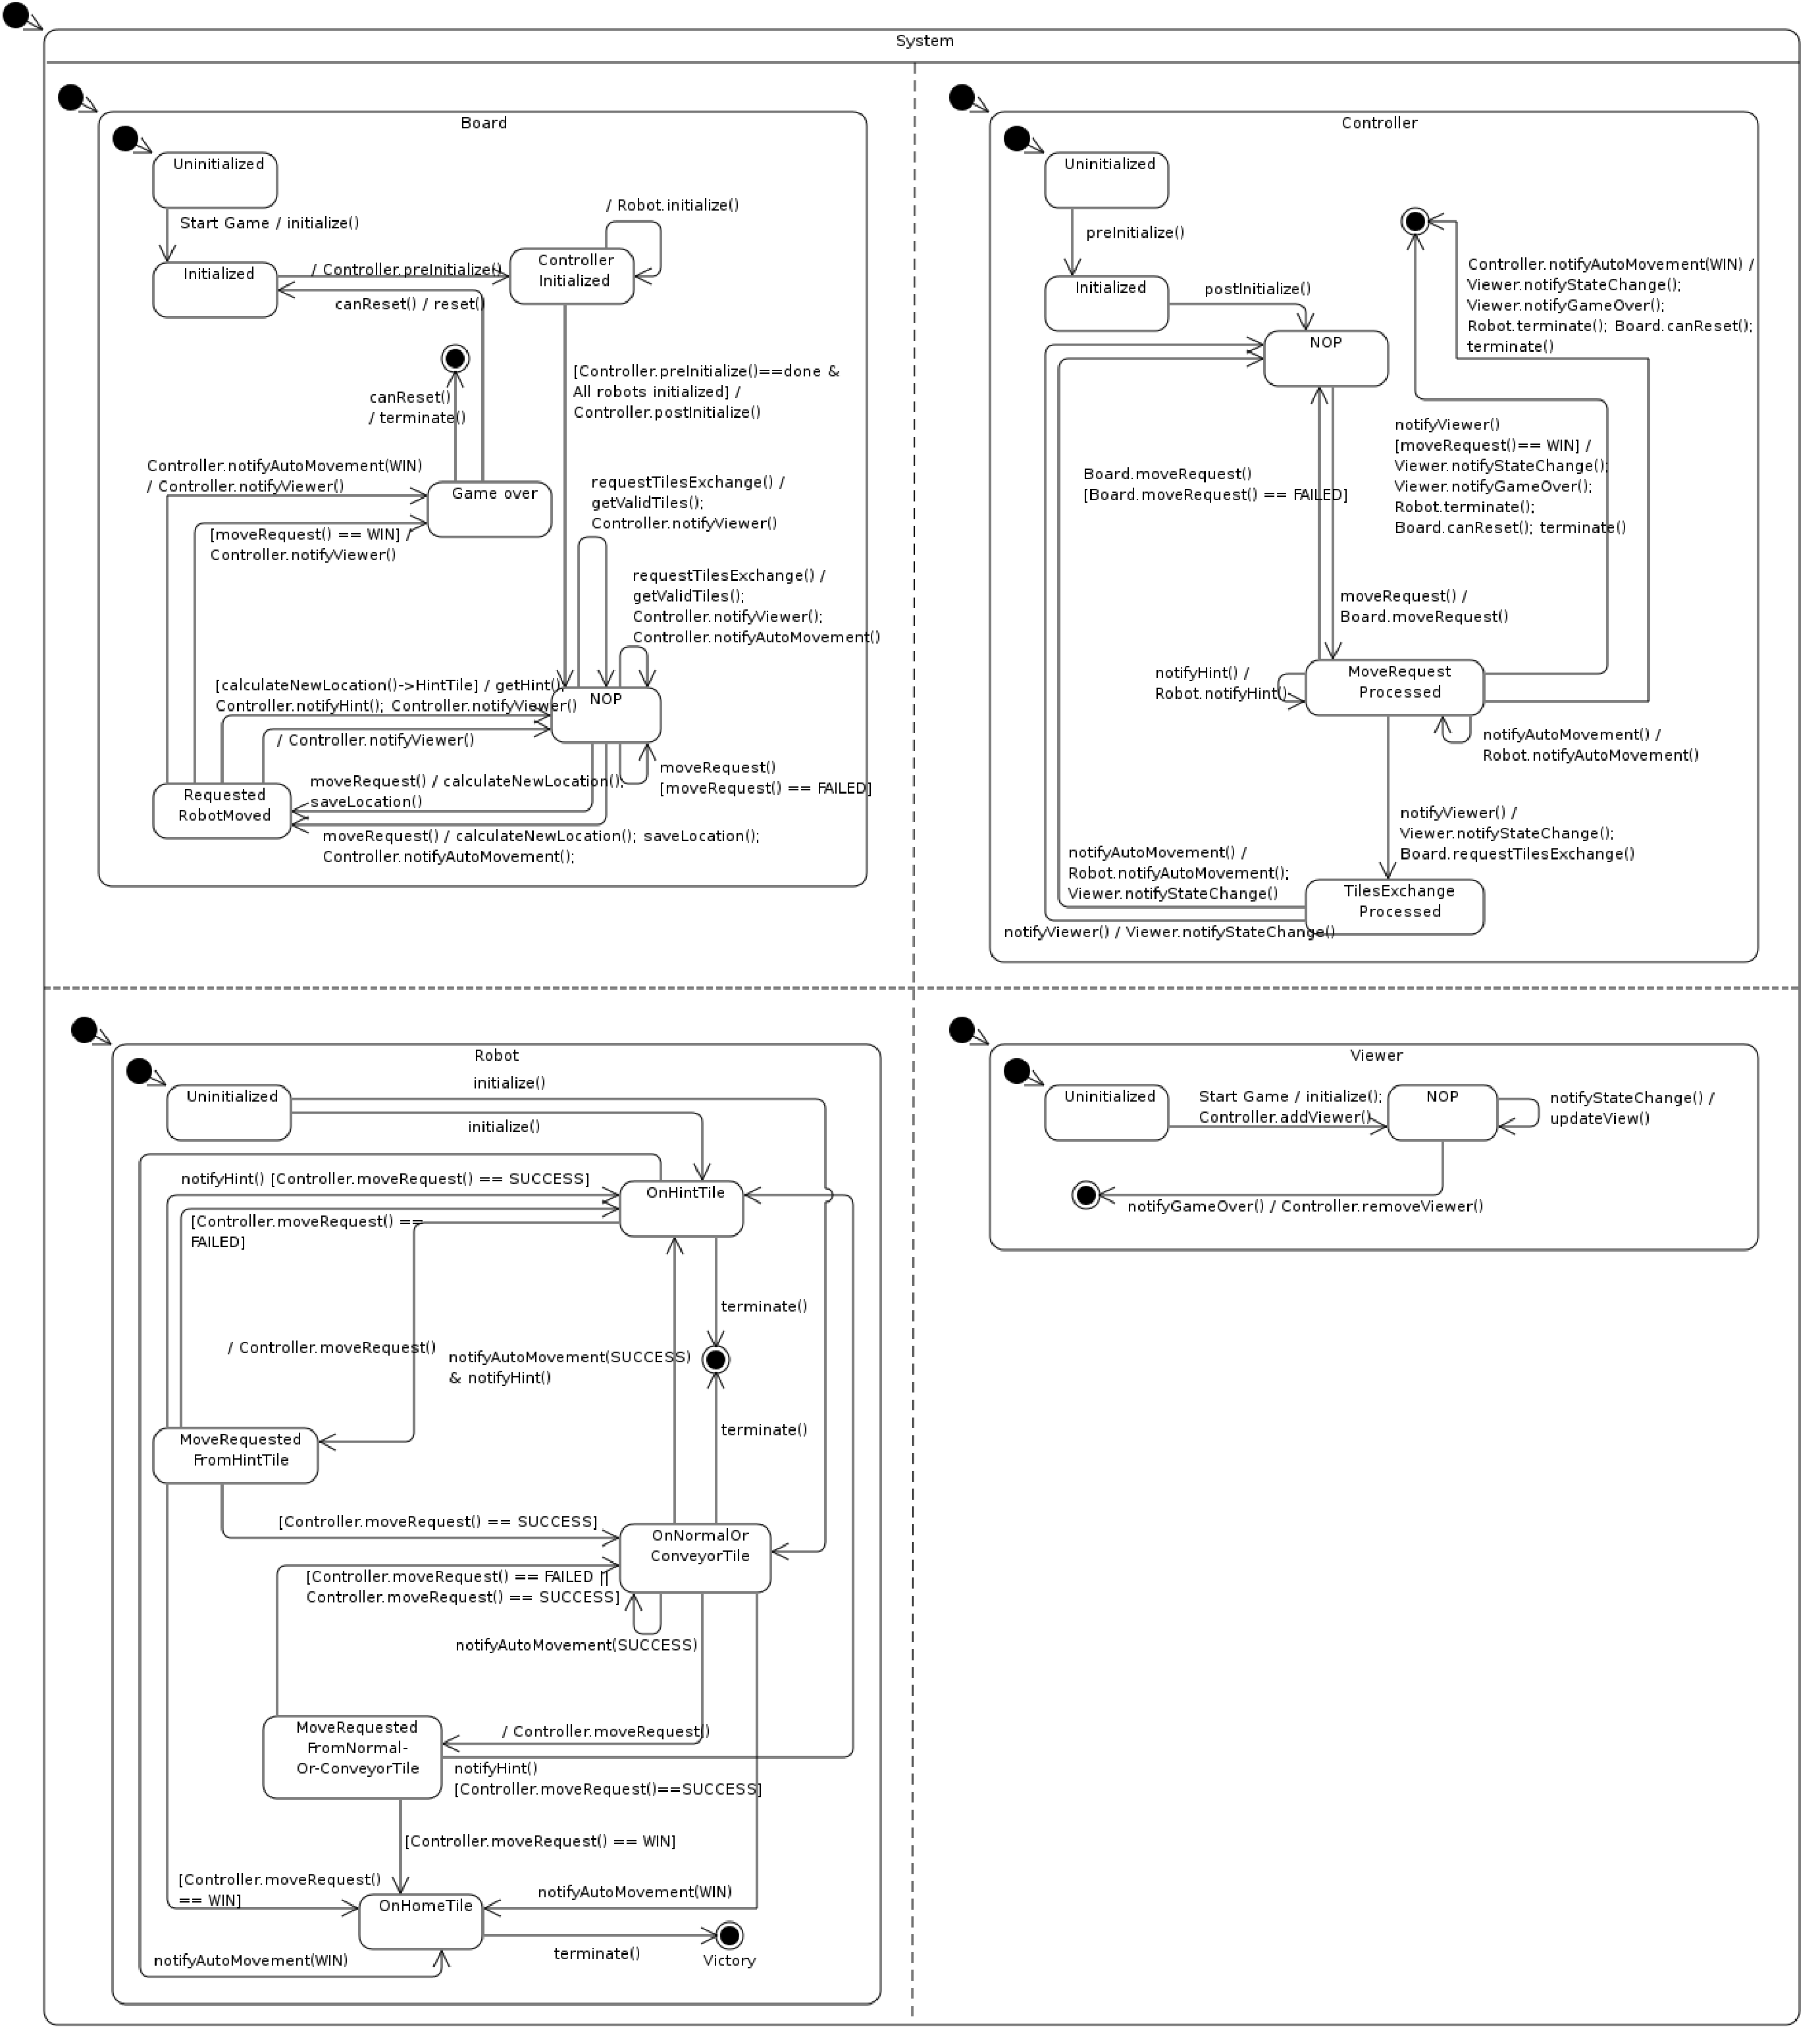
\includegraphics[width=\linewidth]{statecharts/system.pdf}

\subsection{Class level}
	\subsubsection{Board}
	Once the board is initialized, it waits until the controller is intialized and then it can start fulfilling tile swap and move requests.
	
	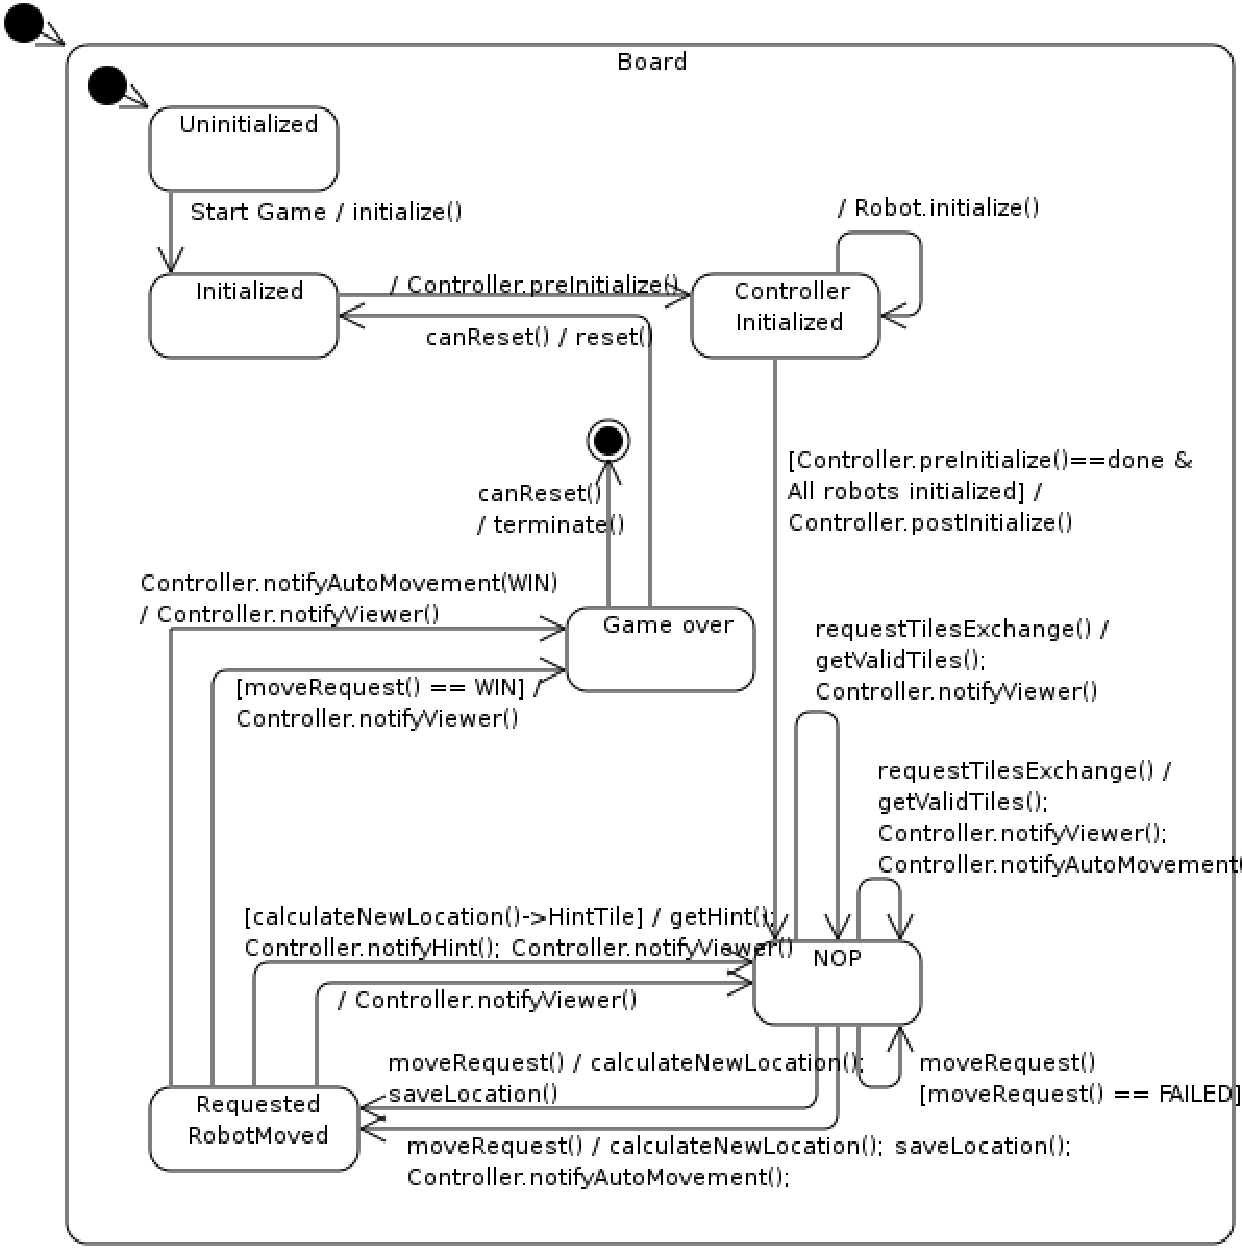
\includegraphics[width=\linewidth]{statecharts/board.pdf}

	\subsubsection{Controller}
	Once the controller is pre- and postInitialized, it can start forwarding messaged between the board and the players.

	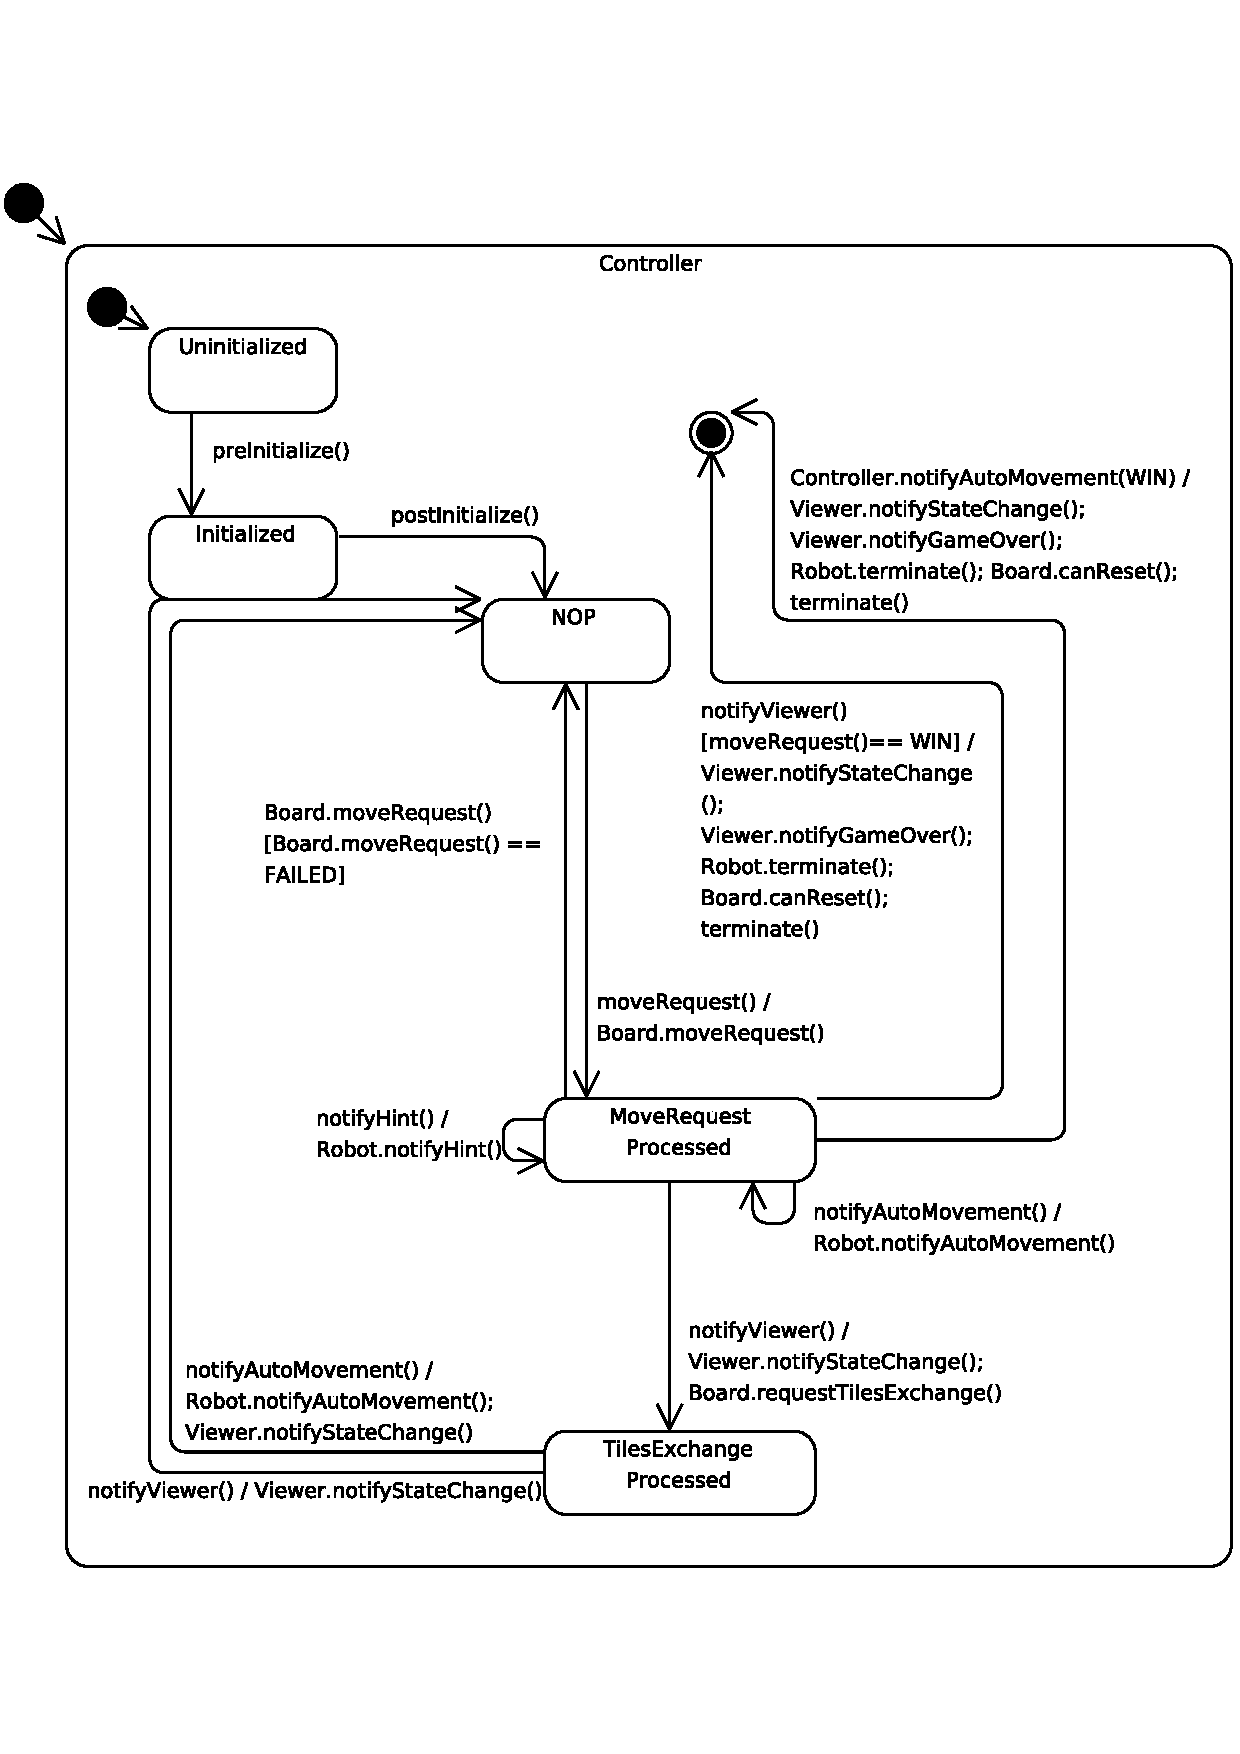
\includegraphics[width=\linewidth]{statecharts/controller.pdf}

	\subsubsection{View}
	Once initialized, the view can request the board status from its NOP (No OPeration) state. It will also request the board status when it is notified that the board status has changed.
	
	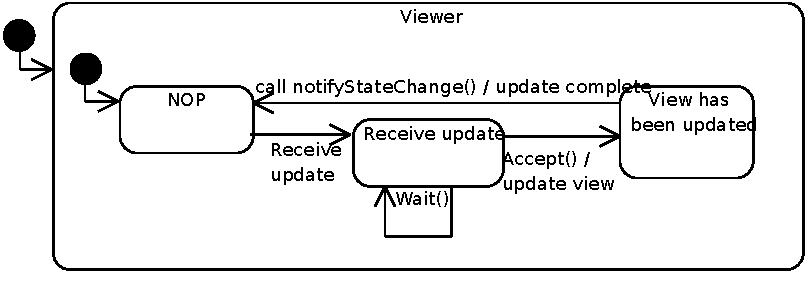
\includegraphics[width=\linewidth]{statecharts/view.pdf}

	\subsubsection{Robot}
	-
	
	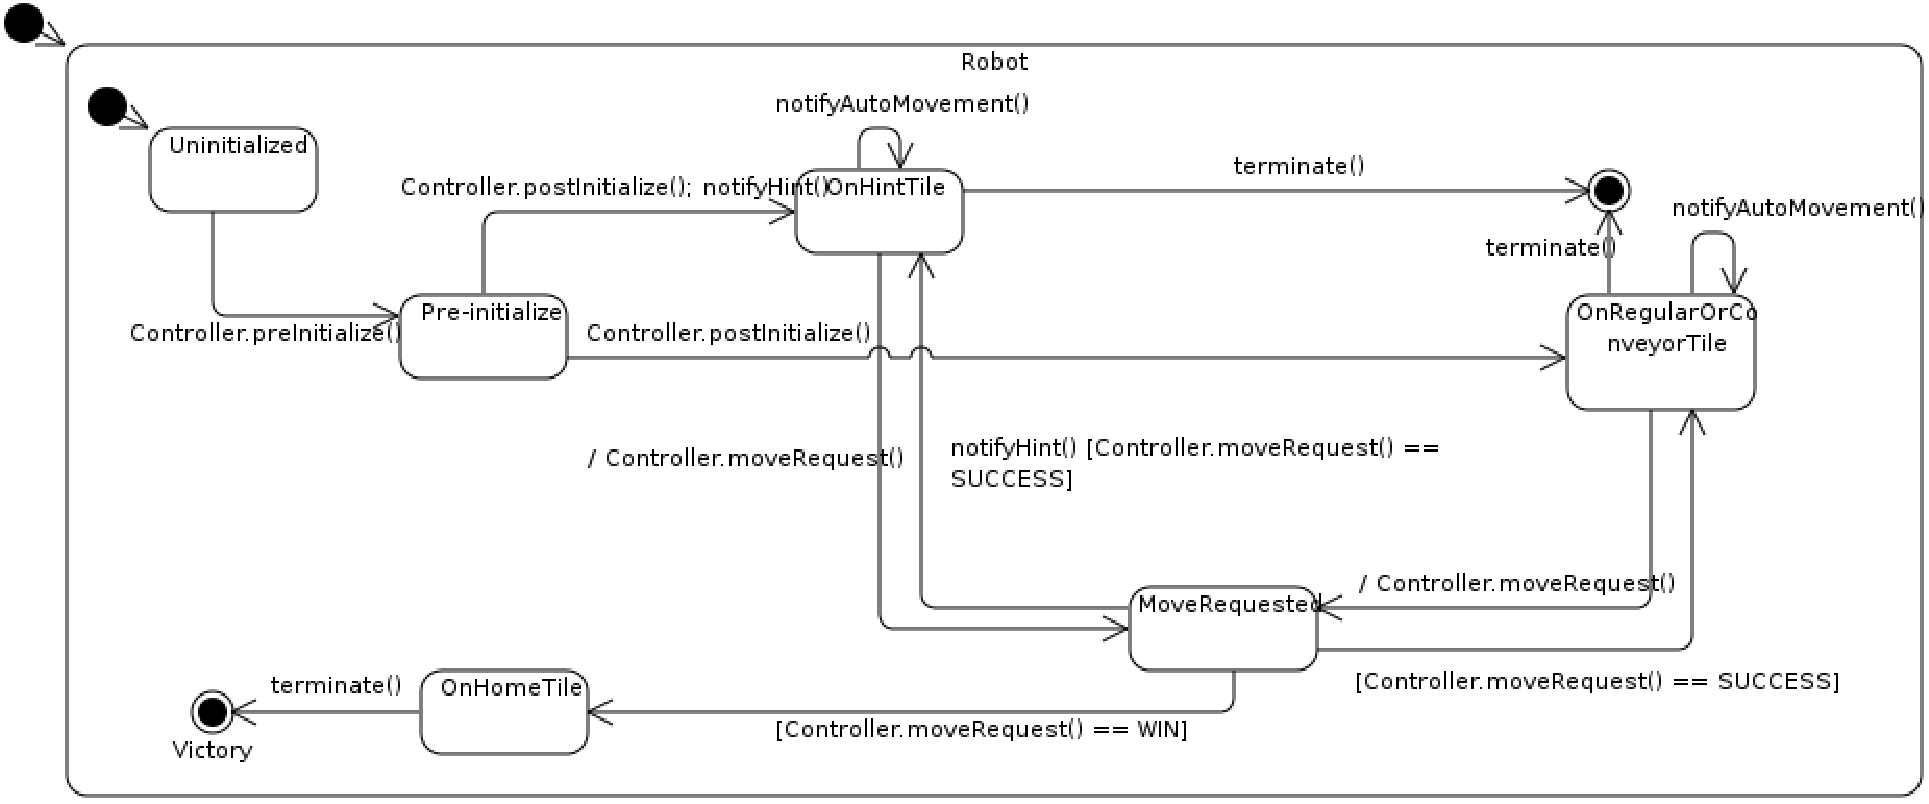
\includegraphics[width=\linewidth]{statecharts/robot.pdf}
	

	
